\chapter{The Faculty of Computer Science}

The \emph{Andreas-Pfitzmann-Bau} (APB in short) houses the Faculty of Computer Science and will therefore be your second home for the next few years. As the number of semesters increases, you will be shooed around the campus less and less and more events will take place here. But what does this building actually have to offer besides a lot of green paint and the sculpture in the foyer?

\begin{figure}[h!]
    \centering
    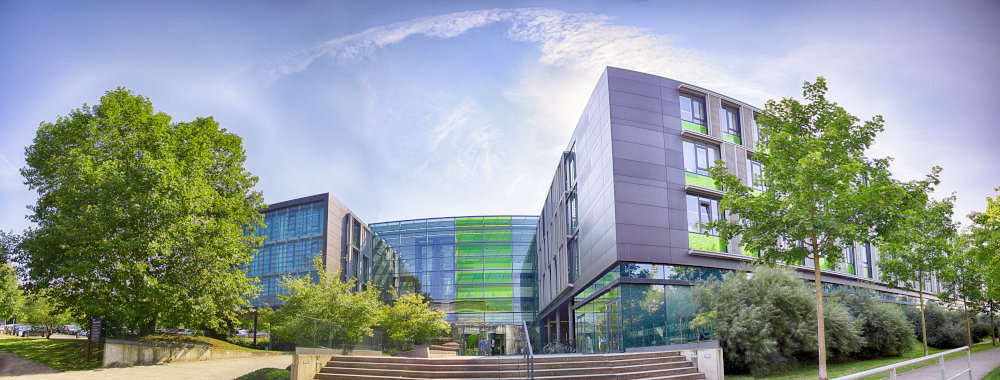
\includegraphics[width=\linewidth]{img/panorama_fakultaet1.jpg}
    \caption*{\small \textit{Der Andreas-Pfitzmann-Bau von vorn -- Foto: Lucas Vogel}}
\end{figure}

One difference between this building and the others on campus is that it is open around the clock. Even if the doors are locked at night, the security service will be happy to open the door for you upon presentation of your student ID and, if you wish, unlock one of the seminar rooms on the first floor.

There is plenty of space to sit in the corridors of all floors, for example to prepare for upcoming exams with your study groups. Furthermore, there are several PC pools, some of which are equipped with special software, but which are only open during the day.

\label{sec:apb}
We also have a large outdoor area. Due to a construction project, however, the pond and the sunbathing lawn are unfortunately not very inviting at the moment.

\begin{figure}[t]
    \centering
    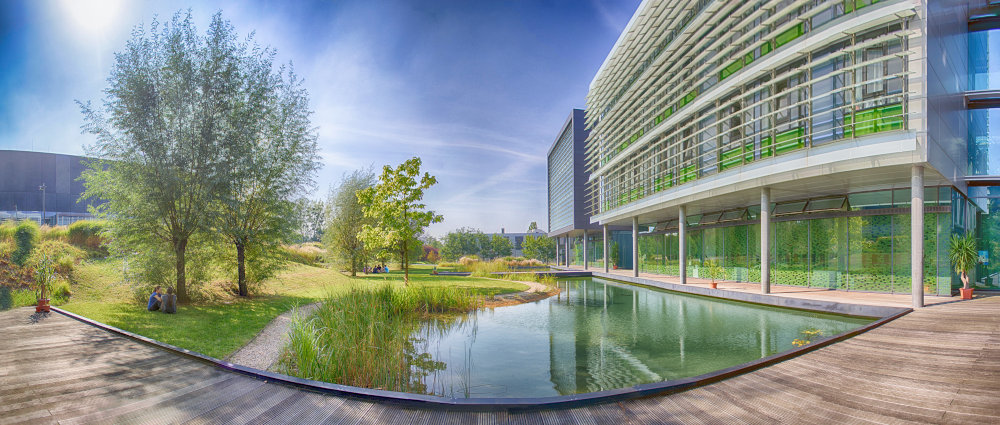
\includegraphics[width=\linewidth]{img/panorama_teich1.jpg}
    \caption*{\small \textit{Der Außenbereich bevor die Bagger kamen -- Foto: Lucas Vogel}}
\end{figure}

This idyll had to give way to a construction site for the time being, as a new building is being erected behind the APB. In addition to many members of the faculty, also your student representatives campaigned for the preservation of the outdoor area with the \href{https://savethetei.ch/}{\#SaveTheTeich campaign}.
The great commitment and tough negotiations paid off: the pond is to be largely restored after the end of construction. To compensate for the lost space on the current slope, above-average funds have now been earmarked for equipping the remaining areas with seats and sufficient greenery. We all hope that the outdoor area will soon shine in new splendor, invite you to take a break and serve as a cozy meeting place again.

From the APB you can see the Rechenzentrum (\enquote{Lehmann-Zentrum}). Maybe you'll get the chance to take part in one of the guided tours through the Rechenzentrum that are offered at various events.

By the way, the building takes its name from Andreas Pfitzmann, one of our professors who died in 2010. For many years, he headed the Chair of Data Protection and Data Security, where he was instrumental in researching ways to make data anonymous, thus enabling many people in countries with censorship and state surveillance to freely access the Internet. In 2009, he also became dean of our faculty. In the foyer you will find a plaque commemorating him and his life's work.

\pagebreak

\minisec{\textbf{ascii} – The café in the faculty}

Since 2007 \ascii{} is located in the building of the Faculty of Computer Science. It is a café run by students who spend a few hours of their free time behind the counter.

The \ascii{} has everything a real café needs: coffee, tea, a variable assortment of savory as well as sweet drinks and of course caffeinated cold drinks. In addition, \ascii{} is one of the few places on campus where you can get Club Mate as well as Kolle Mate and Premium Cola.

\begin{figure}[h!]
    \centering
    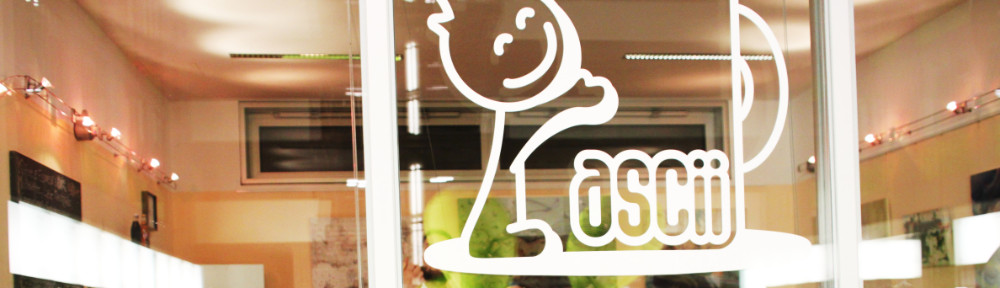
\includegraphics[width=\linewidth]{img/ascii.jpg}
\end{figure}

The \ascii{} is run by a student association and has been a central contact point at the faculty since its founding. Students and employees meet here to spend their breaks, work or simply replenish their caffeine supply. On the comfortable sofas you can let time pass by, work together on projects, learn, program or just chat with fellow students.

If you now feel like visiting ascii or even joining as a member yourself, just drop by and say hello!

For more information, visit~\link{https://www.ascii-dresden.de/}.

\begin{awesomeblock}[ese_bg_color]{2pt}{\faCalendar*[regular]}{ese_bg_color}
    \textbf{Opening hours during the semester}

    Monday to Thursday: 9 a.m. to 5 p.m.

    Fridays: 9 a.m. to 3 p.m.
\end{awesomeblock}
